%!TEX root = head.tex

\section{Empirical Validation}
\label{sec:exp}

To demonstrate the practical value of the theory developed in the previous
sections, we argue that our symbolic refinement-checking algorithms
\begin{itemize}

  \item scale far beyond existing algorithms, and

  \item are often complete in practice.

\end{itemize}
To argue these points we have implemented several variations of three basic
refinement-checking algorithms.

\begin{description}

  \item[{\sc Enumerate}] checks each history $h$ by enumerating the
  linearizations $h'$ of $h$'s completions. We check whether each $h'$ is
  included in the kernel $H$ by asking\footnote{Classically this check is
  performed by set inclusion, as the length of $h$ is assumed to be bounded by
  some number $n \in \<Nats>$ of operations, and the subset $H_n \subseteq H$
  of $n$-operation histories of $H$ is computable in finite time. As we assume
  no such bound on the number of operations, we perform this check via
  theorem-prover query instead.} whether $h' |= \textsc{Theory}(H)$. As soon as
  this check succeeds, we conclude that $h \in \overline{H}$. Otherwise if this
  check fails for all linearizations $h'$, we conclude $h \not\in
  \overline{H}$. We also implement a variation which skips the enumeration of
  $h$'s completions, allowing the solver to search the space of completions
  symbolically. The {\tt -c} flag specifies explicit enumeration of completions.

  \item[{\sc Symbolic}] checks each history $h$ by reduction to the
  satisfiability of $\textsc{Stronger}(h) /| \textsc{Theory}(H)$, as described
  in Section~\ref{sec:propositional}, delegating the enumeration of both
  completions and linearizations to an underlying solver. If the satisfiability
  check succeeds, or is inconclusive, we conclude that $h \in \overline{H}$.
  Otherwise if unsatisfiability is found, we conclude that $h \not\in
  \overline{H}$. We also implement variations where the completions of $h'$ are
  enumerated explicitly ({\tt -c}), where the formula $\textsc{Stronger}(h)$ is
  asserted to the solver incrementally as operations begin and end ({\tt -i}),
  where the match-removal optimization of Section~\ref{sec:obsolete} is
  performed ({\tt -r}), and any combination of the three.

  \item[{\sc Saturate}] avoids the expensive propositional backtracking
  inherent to the aforementioned {\sc Symbolic} checker by limiting the
  satisfiability check to Boolean constraint propagation. Essentially, we
  implement a customized incremental solver which only saturates with unit
  propagation, avoiding any propositional branching. If a contradiction is
  found, we conclude that $h \not\in \overline{H}$. Otherwise if saturation
  fails to reveal a contradiction, we conclude $h \in \overline{H}$. We also
  implement a variation where the match-removal optimization of
  Section~\ref{sec:obsolete} is performed ({\tt -r}).

\end{description}

We have studied actual concurrent data structure implementations, including the
Scal\footnote{\url{http://scal.cs.uni-salzburg.at}} High-Performance
Multicore-Scalable Computing suite. Some of these implementations, such as the
Michael-Scott Queue~\cite{conf/podc/MichaelS96}, are meant to preserve
observational refinement\footnote{More precisely, they are designed to be
linearizable.}, while others, such as the non-blocking bounded-reordering
queue~\cite{conf/pact/KirschLP13}, are meant to preserve weaker properties.

The input to our checking algorithms are histories given as text files
consisting of line-separated call and return actions. For the selected set of
concurrent object implementations, we generated the histories of several
executions under pseudo-random scheduling by logging calls and returns in the
order in which they occurred. While scanning an input history, the selected
algorithm performs a membership test at each prefix at which an operation
completes --- i.e.,~at return actions.

Our first set of experiments (\S\ref{sec:exp:scalable}) demonstrates that our
symbolic algorithms are drastically more scalable than existing algorithms, in
that they are able to process vastly more history operations in much shorter
time. Our second set of experiments (\S\ref{sec:exp:complete}) demonstrates
that while our more efficient algorithms can be incomplete on certain
hand-crafted cases, failing to identify particularly intricate refinement
violations, the violations surfacing in the logs of actual executions are
consistently discovered. We made all measurements on similar MacBook Pro 2.XGHz
Intel Core i5/i7 machines, and discharged theorem-prover queries with an
in-process instance of Z3 compiled from revision {\tt cee7dd3}.

% YOU WANT THE LINK??? YOU CAN'T HANDLE THE LINK!!!
% \footnote{\url{http://z3.codeplex.com/SourceControl/changeset/cee7dd39444c9060186df79c2a2c7f8845de415b}}

Our implementation of the algorithms, and all (generated) histories used in
these experiments, are available on
Github\footnote{\url{https://github.com/pldi15-anonymous/refinement-monitor-experiments}}.

\subsection{Scalability of Symbolic Checking}
\label{sec:exp:scalable}

Our first experiment measures the number of steps each algorithm is able to
process for varying time limits, averaged over $10$ histories of an atomic
stack implementation with an average of $1020.8$ steps. We used five
per-history time limits of $5$s, $25$s, $50$s, $75$s, and $100$s. The graph of
Figure~\ref{fig:steprace} shows the results with time plotted on the y-axis,
and number of steps plotted on the x-axis on a logarithmic scale. The {\sc
Enumerate} algorithm performs worst, progressing only from $16$ steps in $5$s to
$18$ steps in $100$s. The {\sc Symbolic} algorithm is a significant improvement,
progressing from $31.6$ steps in $5$s to $52.7$ steps in $100$s. While adding match
removal helps, achieving roughly an order-of-magnitude improvement over {\sc
Enumerate}, the cost of checking remains exponential in the number of steps.

\begin{figure}[t]
  \centering
  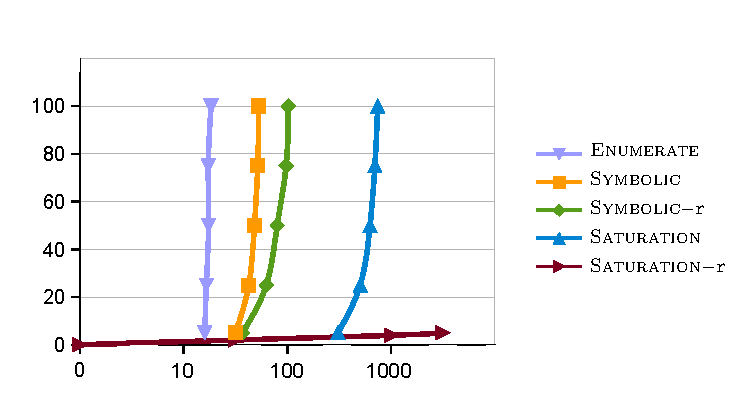
\includegraphics[width=\linewidth]{figures/chart_efficiency}
  \caption{The number of steps each algorithm is able to process in given time
  limits of $5$s, $25$s, $50$s, $75$s, and $100$s, per history averaged over
  $10$ histories of an atomic stack implementation. Further right is better.
  The x-axis plots steps on a logarithmic scale, and the y-axis plots time.}
  \label{fig:steprace}
\end{figure}

Even without match removal, the {\sc Saturate} checker achieves roughly a
two-orders-of-magnitude improvement over {\sc Enumerate}, progressing from $307.7$
steps in $5$s to $744.6$ steps in $100$s. Most impressively, adding match removal
to the {\sc Saturate} checker allows it to process \emph{all} $1020.8$ steps in
under $5$s.

Our second experiment measures the average number of steps each algorithm is
able to process in a fixed time limit of $5$s per history over $100$ histories
of Scal's Michael-Scott Queue and $100$ histories of Scal's bounded-reordering
queue. Each history contains $20$ {\sf enqueue}-operations and $30$ {\sf
dequeue} operations (total $100$ steps) obtained from highly-concurrent
executions in which most operations are concurrent. Although most sequential
executions of the bounded-reordering queue exhibit violations with respect to
an atomic queue, the extreme concurrency in this set of histories allows great
freedom in the linearization of operations, rendering all but $4$ histories
violation free. Table~\ref{tab:exp:con} shows the results, including the
average number of steps (out of $100$) processed, and the number of violations
(out of $4$) discovered, within the $5$s time limit. While the {\sc Enumerate}
algorithm is never able to process enough steps in $5$s to detect any of the
violations, the {\sc Symbolic} checker, at least without computing history
completions, does detect $3$ out of $4$ violations. Once again, the {\sc
Saturate} checker swiftly processes all histories to their entirety well under
the time limit, averaging $0.1$s, correctly detecting all $4$ violations.

\begin{table}[t]
  \footnotesize
  \centering
  \setlength{\tabcolsep}{1.8mm}
  \begin{tabular}{lcccc}
    Algorithm & Avg. steps & Avg. time & Nb. violations \\
    \hline
    {\sc Enumerate}             & 35  & --      & 0/4 \\
    {\sc Enumerate} {\tt -c}    & 38  & --      & 0/4 \\
    {\sc Symbolic}              & 52  & --      & 3/4 \\
    {\sc Symbolic} {\tt -r}     & 52  & --      & 3/4 \\
    {\sc Symbolic} {\tt -i}     & 51  & --      & 3/4 \\
    {\sc Symbolic} {\tt -c}     & 38  & --      & 0/4 \\
    {\sc Symbolic} {\tt -c -i}  & 38  & --      & 0/4 \\
    {\sc Saturate}              & 100 & 0.1340s & 4/4 \\
    {\sc Saturate} {\tt -r}     & 100 & 0.1521s & 4/4
  \end{tabular} 

  \caption{The average number of steps each algorithm is able to process in a
  fixed time limit of $5$s per history, averaged over $200$ very-concurrent
  histories.}
  \label{tab:exp:con}
\end{table}


\subsection{Completeness in Practice}
\label{sec:exp:complete}

While the second experiment of Table~\ref{tab:exp:con} already demonstrates
that ``needle-in-a-haystack'' violations are swiftly discovered by the {\sc
Saturate} checker, our third experiment elaborates, measuring the percentage of
violations each algorithm is able discover in a fixed time limit of $5$s per
history over $100$ histories of Scal's bounded-reordering queue. Each history
contains $20$ {\sf enqueue}-operations and $30$ {\sf dequeue} operations (total
$100$ steps) obtained from highly-sequential executions in which most
operations are sequential. Consequently, the extreme sequentiality in this set
of histories greatly limits freedom in the linearization of operations of the
reordering queue, rendering all $100$ histories violations.
Table~\ref{tab:exp:seq} shows the results, including the percentage of
histories in which, and average step at which, the violation was discovered
within the $5$s time limit. Since most operations are already ordered, the {\sc
Enumerate} checker has very few completions and linearizations to perform, and
succeeds in exposing most, but not all violations. The {\sc Symbolic} checker
is more efficient, particularly when interacting with the solver incrementally,
and computing completions explicitly. Still, the {\sc Saturate} checker is far
more efficient, and succeeds in discovering \emph{every} violation. Notice that
in some cases the {\sc Saturate} checker requires more steps to detect a
violation. This is of course by design, as we wish to avoid branching and
backtracking on the possible completions of operations.

\begin{table}[t]
  \footnotesize
  \centering
  \setlength{\tabcolsep}{1.8mm}
  \begin{tabular}{lccc}
   	          & 	              & Avg. step \\
    Algorithm & $\%$ violations & detected  \\
    \hline
    {\sc Enumerate}             & 55$\%$  & 23.8 \\
    {\sc Enumerate} {\tt -c}    & 88$\%$  & 23.8 \\
    {\sc Symbolic}              & 75$\%$  & 23.8 \\
    {\sc Symbolic} {\tt -r}     & 78$\%$  & 23.8 \\
    {\sc Symbolic} {\tt -i}     & 90$\%$  & 23.8 \\
    {\sc Symbolic} {\tt -c}     & 100$\%$ & 23.8 \\
    {\sc Symbolic} {\tt -c -i}  & 100$\%$ & 23.8 \\
    {\sc Saturate}              & 100$\%$ & 24.2 \\
    {\sc Saturate} {\tt -r}     & 100$\%$ & 24.2
  \end{tabular} 

  \caption{The percentage of violations each algorithm is able to discover in a
  fixed time limit of $5$s per history, over $100$ barely-concurrent histories.}
  \label{tab:exp:seq}
\end{table}

Finally, we address the possible sources of incompleteness due to match removal
discussed in Section~\ref{sec:obsolete}. Recall the history $h$ and its
extension $h'$ of Figure~\ref{fig:removal_no_saturation} from
Example~\ref{ex:removal_no_saturation}. Since the {\sc Saturate} algorithm does
not speculate on whether the pending {\sf rem}-operation might match the {\sf
add} of $2$ or $3$ (or both!), it will not detect the violation in $h$ until
the pending {\sf rem}-operation completes. Simply removing the {\sf add}-{\sf
rem} match of value $1$ from $h$ before the pending {\sf rem}-operation
completes would result in a non-violating history. However, by applying the
stack-theory axioms $\textsc{Theory}(H_{\sf st})$ to completed operations
before removing this match, the {\sc Saturate} algorithm infers the constraints
\begin{align*}
  {\sf add}(2) < {\sf add}(1) < ({\sf rem} => 1) < ({\sf rem} => {\tt empty})
\end{align*}
of which ${\sf add}(2) < ({\sf rem} => {\tt empty})$ persists after the
match removal. Finally, when the pending {\sf rem}-operation does complete,
returning $2$, the {\sc Saturate} algorithm derives a contradiction, since
\begin{align*}
  {\sf add}(2) < ({\sf rem} => {\tt empty}) < ({\sf rem} => 2).
\end{align*}
The incremental nature of the {\sc Saturate} algorithm thus avoids the
practically-occurring sources of possible incompleteness due to match removal
of which we are aware.
